\providecommand{\Person}[1]{
\draw[ultra thick] (#1) circle (.4cm);
}
\providecommand{\Exposed}[1]{
\draw[ultra thick,fill=gray!50] (#1) circle (.4cm);
}
\providecommand{\Sick}[1]{
\draw[ultra thick] (#1) -- +(.25,.25);
\draw[ultra thick] (#1) -- +(.25,-.25);
\draw[ultra thick] (#1) -- +(-.25,-.25);
\draw[ultra thick] (#1) -- +(-.25,.25);
}
\providecommand{\PersonSick}[1]{
\Person{#1}
\Sick{#1}
}
\providecommand{\ExposedSick}[1]{
\Exposed{#1}
\Sick{#1}
}

The diagrams below show different diseases along with exposure to
some hypothesized cause.  

{\bf Key}: Each circle is a person who might or might not have been exposed to the hypothetical cause and who might or might not have eventually acquired the disease.
\begin{itemize}
\item Exposed but not sick 
\begin{tikzpicture} \Exposed{0,0} \end{tikzpicture}
\item Sick 
\begin{tikzpicture} \PersonSick{0,0} \end{tikzpicture}
\item Exposed and Sick 
\begin{tikzpicture} \ExposedSick{0,0} \end{tikzpicture}
\item Neither exposed nor sick 
\begin{tikzpicture} \Person{0,0} \end{tikzpicture}
\end{itemize}


For each of the diseases, say whether the
exposure is a necessary and/or sufficient cause for development of the disease.

\begin{itemize}
\item Disease A


\begin{tikzpicture}
\Person{0,0}\ExposedSick{0,1}\ExposedSick{0,2}\Person{0,3}\Person{0,4}\Person{0,5}
\Person{1,0}\ExposedSick{1,1}\Person{1,2}\Person{1,3}\ExposedSick{1,4}\Person{1,5}
\ExposedSick{2,0}\Person{2,1}\Person{2,2}\ExposedSick{2,3}\ExposedSick{2,4}\Person{2,5}
\ExposedSick{3,0}\Person{3,1}\ExposedSick{3,2}\Person{3,3}\ExposedSick{3,4}\ExposedSick{3,5}
\Person{4,0}\Person{4,1}\Person{4,2}\ExposedSick{4,3}\Person{4,4}\Person{4,5}
\ExposedSick{5,0}\Person{5,1}\Person{5,2}\ExposedSick{5,3}\Person{5,4}\ExposedSick{5,5}
\end{tikzpicture}

For Disease A
\begin{MultipleChoice}[itemname=nec-and-suff-a]
\wrong{Necessary but not sufficient}
\wrong{Sufficient but not necessary}
\correct{Necessary and Sufficient}
\wrong{Neither necessary nor sufficient}
\end{MultipleChoice}

\end{itemize}

\begin{itemize}
\item Disease B

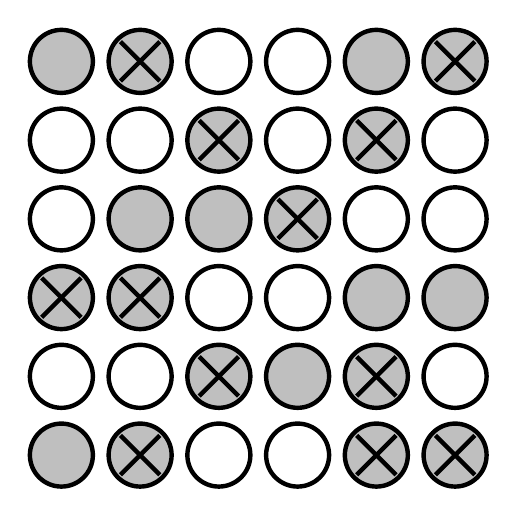
\begin{tikzpicture}
\Exposed{0,0}\Person{0,1}\ExposedSick{0,2}\Person{0,3}\Person{0,4}\Exposed{0,5}
\ExposedSick{1,0}\Person{1,1}\ExposedSick{1,2}\Exposed{1,3}\Person{1,4}\ExposedSick{1,5}
\Person{2,0}\ExposedSick{2,1}\Person{2,2}\Exposed{2,3}\ExposedSick{2,4}\Person{2,5}
\Person{3,0}\Exposed{3,1}\Person{3,2}\ExposedSick{3,3}\Person{3,4}\Person{3,5}
\ExposedSick{4,0}\ExposedSick{4,1}\Exposed{4,2}\Person{4,3}\ExposedSick{4,4}\Exposed{4,5}
\ExposedSick{5,0}\Person{5,1}\Exposed{5,2}\Person{5,3}\Person{5,4}\ExposedSick{5,5}
\end{tikzpicture}

For Disease B
\begin{MultipleChoice}[itemname=nec-and-suff-b]
\wrong{Necessary but not sufficient}
\correct{Sufficient but not necessary}
\wrong{Necessary and Sufficient}
\wrong{Neither necessary nor sufficient}
\end{MultipleChoice}

\end{itemize}

